\documentclass{ximera}  


%\usepackage{todonotes}
%\usepackage{mathtools} %% Required for wide table Curl and Greens
%\usepackage{cuted} %% Required for wide table Curl and Greens
\newcommand{\todo}{}

\usepackage{esint} % for \oiint
\ifxake%%https://math.meta.stackexchange.com/questions/9973/how-do-you-render-a-closed-surface-double-integral
\renewcommand{\oiint}{{\large\bigcirc}\kern-1.56em\iint}
\fi


\graphicspath{
  {./}
  {jpg}
  {ximeraTutorial/}
  {basicPhilosophy/}
  {functionsOfSeveralVariables/}
  {normalVectors/}
  {lagrangeMultipliers/}
  {vectorFields/}
  {greensTheorem/}
  {shapeOfThingsToCome/}
  {dotProducts/}
  {partialDerivativesAndTheGradientVector/}
  {../productAndQuotientRules/exercises/}
  {../motionAndPathsInSpace/exercises/}
  {../normalVectors/exercisesParametricPlots/}
  {../continuityOfFunctionsOfSeveralVariables/exercises/}
  {../partialDerivativesAndTheGradientVector/exercises/}
  {../directionalDerivativeAndChainRule/exercises/}
  {../commonCoordinates/exercisesCylindricalCoordinates/}
  {../commonCoordinates/exercisesSphericalCoordinates/}
  {../greensTheorem/exercisesCurlAndLineIntegrals/}
  {../greensTheorem/exercisesDivergenceAndLineIntegrals/}
  {../shapeOfThingsToCome/exercisesDivergenceTheorem/}
  {../greensTheorem/}
  {../shapeOfThingsToCome/}
  {../separableDifferentialEquations/exercises/}
  {vectorFields/}
}

\newcommand{\mooculus}{\textsf{\textbf{MOOC}\textnormal{\textsf{ULUS}}}}

\usepackage{tkz-euclide}\usepackage{tikz}
\usepackage{tikz-cd}
\usetikzlibrary{arrows}
\tikzset{>=stealth,commutative diagrams/.cd,
  arrow style=tikz,diagrams={>=stealth}} %% cool arrow head
\tikzset{shorten <>/.style={ shorten >=#1, shorten <=#1 } } %% allows shorter vectors

\usetikzlibrary{backgrounds} %% for boxes around graphs
\usetikzlibrary{shapes,positioning}  %% Clouds and stars
\usetikzlibrary{matrix} %% for matrix
\usepgfplotslibrary{polar} %% for polar plots
\usepgfplotslibrary{fillbetween} %% to shade area between curves in TikZ
\usetkzobj{all}
\usepackage[makeroom]{cancel} %% for strike outs
%\usepackage{mathtools} %% for pretty underbrace % Breaks Ximera
%\usepackage{multicol}
\usepackage{pgffor} %% required for integral for loops



%% http://tex.stackexchange.com/questions/66490/drawing-a-tikz-arc-specifying-the-center
%% Draws beach ball
\tikzset{pics/carc/.style args={#1:#2:#3}{code={\draw[pic actions] (#1:#3) arc(#1:#2:#3);}}}



\usepackage{array}
\setlength{\extrarowheight}{+.1cm}
\newdimen\digitwidth
\settowidth\digitwidth{9}
\def\divrule#1#2{
\noalign{\moveright#1\digitwidth
\vbox{\hrule width#2\digitwidth}}}





\newcommand{\RR}{\mathbb R}
\newcommand{\R}{\mathbb R}
\newcommand{\N}{\mathbb N}
\newcommand{\Z}{\mathbb Z}

\newcommand{\sagemath}{\textsf{SageMath}}


%\renewcommand{\d}{\,d\!}
\renewcommand{\d}{\mathop{}\!d}
\newcommand{\dd}[2][]{\frac{\d #1}{\d #2}}
\newcommand{\pp}[2][]{\frac{\partial #1}{\partial #2}}
\renewcommand{\l}{\ell}
\newcommand{\ddx}{\frac{d}{\d x}}

\newcommand{\zeroOverZero}{\ensuremath{\boldsymbol{\tfrac{0}{0}}}}
\newcommand{\inftyOverInfty}{\ensuremath{\boldsymbol{\tfrac{\infty}{\infty}}}}
\newcommand{\zeroOverInfty}{\ensuremath{\boldsymbol{\tfrac{0}{\infty}}}}
\newcommand{\zeroTimesInfty}{\ensuremath{\small\boldsymbol{0\cdot \infty}}}
\newcommand{\inftyMinusInfty}{\ensuremath{\small\boldsymbol{\infty - \infty}}}
\newcommand{\oneToInfty}{\ensuremath{\boldsymbol{1^\infty}}}
\newcommand{\zeroToZero}{\ensuremath{\boldsymbol{0^0}}}
\newcommand{\inftyToZero}{\ensuremath{\boldsymbol{\infty^0}}}



\newcommand{\numOverZero}{\ensuremath{\boldsymbol{\tfrac{\#}{0}}}}
\newcommand{\dfn}{\textbf}
%\newcommand{\unit}{\,\mathrm}
\newcommand{\unit}{\mathop{}\!\mathrm}
\newcommand{\eval}[1]{\bigg[ #1 \bigg]}
\newcommand{\seq}[1]{\left( #1 \right)}
\renewcommand{\epsilon}{\varepsilon}
\renewcommand{\phi}{\varphi}


\renewcommand{\iff}{\Leftrightarrow}

\DeclareMathOperator{\arccot}{arccot}
\DeclareMathOperator{\arcsec}{arcsec}
\DeclareMathOperator{\arccsc}{arccsc}
\DeclareMathOperator{\si}{Si}
\DeclareMathOperator{\scal}{scal}
\DeclareMathOperator{\sign}{sign}


%% \newcommand{\tightoverset}[2]{% for arrow vec
%%   \mathop{#2}\limits^{\vbox to -.5ex{\kern-0.75ex\hbox{$#1$}\vss}}}
\newcommand{\arrowvec}[1]{{\overset{\rightharpoonup}{#1}}}
%\renewcommand{\vec}[1]{\arrowvec{\mathbf{#1}}}
\renewcommand{\vec}[1]{{\overset{\boldsymbol{\rightharpoonup}}{\mathbf{#1}}}\hspace{0in}}

\newcommand{\point}[1]{\left(#1\right)} %this allows \vector{ to be changed to \vector{ with a quick find and replace
\newcommand{\pt}[1]{\mathbf{#1}} %this allows \vec{ to be changed to \vec{ with a quick find and replace
\newcommand{\Lim}[2]{\lim_{\point{#1} \to \point{#2}}} %Bart, I changed this to point since I want to use it.  It runs through both of the exercise and exerciseE files in limits section, which is why it was in each document to start with.

\DeclareMathOperator{\proj}{\mathbf{proj}}
\newcommand{\veci}{{\boldsymbol{\hat{\imath}}}}
\newcommand{\vecj}{{\boldsymbol{\hat{\jmath}}}}
\newcommand{\veck}{{\boldsymbol{\hat{k}}}}
\newcommand{\vecl}{\vec{\boldsymbol{\l}}}
\newcommand{\uvec}[1]{\mathbf{\hat{#1}}}
\newcommand{\utan}{\mathbf{\hat{t}}}
\newcommand{\unormal}{\mathbf{\hat{n}}}
\newcommand{\ubinormal}{\mathbf{\hat{b}}}

\newcommand{\dotp}{\bullet}
\newcommand{\cross}{\boldsymbol\times}
\newcommand{\grad}{\boldsymbol\nabla}
\newcommand{\divergence}{\grad\dotp}
\newcommand{\curl}{\grad\cross}
%\DeclareMathOperator{\divergence}{divergence}
%\DeclareMathOperator{\curl}[1]{\grad\cross #1}
\newcommand{\lto}{\mathop{\longrightarrow\,}\limits}

\renewcommand{\bar}{\overline}

\colorlet{textColor}{black}
\colorlet{background}{white}
\colorlet{penColor}{blue!50!black} % Color of a curve in a plot
\colorlet{penColor2}{red!50!black}% Color of a curve in a plot
\colorlet{penColor3}{red!50!blue} % Color of a curve in a plot
\colorlet{penColor4}{green!50!black} % Color of a curve in a plot
\colorlet{penColor5}{orange!80!black} % Color of a curve in a plot
\colorlet{penColor6}{yellow!70!black} % Color of a curve in a plot
\colorlet{fill1}{penColor!20} % Color of fill in a plot
\colorlet{fill2}{penColor2!20} % Color of fill in a plot
\colorlet{fillp}{fill1} % Color of positive area
\colorlet{filln}{penColor2!20} % Color of negative area
\colorlet{fill3}{penColor3!20} % Fill
\colorlet{fill4}{penColor4!20} % Fill
\colorlet{fill5}{penColor5!20} % Fill
\colorlet{gridColor}{gray!50} % Color of grid in a plot

\newcommand{\surfaceColor}{violet}
\newcommand{\surfaceColorTwo}{redyellow}
\newcommand{\sliceColor}{greenyellow}




\pgfmathdeclarefunction{gauss}{2}{% gives gaussian
  \pgfmathparse{1/(#2*sqrt(2*pi))*exp(-((x-#1)^2)/(2*#2^2))}%
}


%%%%%%%%%%%%%
%% Vectors
%%%%%%%%%%%%%

%% Simple horiz vectors
\renewcommand{\vector}[1]{\left\langle #1\right\rangle}


%% %% Complex Horiz Vectors with angle brackets
%% \makeatletter
%% \renewcommand{\vector}[2][ , ]{\left\langle%
%%   \def\nextitem{\def\nextitem{#1}}%
%%   \@for \el:=#2\do{\nextitem\el}\right\rangle%
%% }
%% \makeatother

%% %% Vertical Vectors
%% \def\vector#1{\begin{bmatrix}\vecListA#1,,\end{bmatrix}}
%% \def\vecListA#1,{\if,#1,\else #1\cr \expandafter \vecListA \fi}

%%%%%%%%%%%%%
%% End of vectors
%%%%%%%%%%%%%

%\newcommand{\fullwidth}{}
%\newcommand{\normalwidth}{}



%% makes a snazzy t-chart for evaluating functions
%\newenvironment{tchart}{\rowcolors{2}{}{background!90!textColor}\array}{\endarray}

%%This is to help with formatting on future title pages.
\newenvironment{sectionOutcomes}{}{}



%% Flowchart stuff
%\tikzstyle{startstop} = [rectangle, rounded corners, minimum width=3cm, minimum height=1cm,text centered, draw=black]
%\tikzstyle{question} = [rectangle, minimum width=3cm, minimum height=1cm, text centered, draw=black]
%\tikzstyle{decision} = [trapezium, trapezium left angle=70, trapezium right angle=110, minimum width=3cm, minimum height=1cm, text centered, draw=black]
%\tikzstyle{question} = [rectangle, rounded corners, minimum width=3cm, minimum height=1cm,text centered, draw=black]
%\tikzstyle{process} = [rectangle, minimum width=3cm, minimum height=1cm, text centered, draw=black]
%\tikzstyle{decision} = [trapezium, trapezium left angle=70, trapezium right angle=110, minimum width=3cm, minimum height=1cm, text centered, draw=black]




 
\title{Electrostatic Field} 
\author{Milica Markovic} 
\outcome{Electrostatic fields.}
\begin{document}  
\begin{abstract}  

\end{abstract}  
\maketitle    


\section{Introduction to Electric Field}


\begin{itemize}
\item a bunch of positives (negatives) would repel away from each other.
\item the opposite pieces would attract each other.
\item the net result is a balance! Balance is formed by tight fine mixtures of positives and negatives.
\item there is no attraction/repulsion between them
\end{itemize}
 

What we described is exactly electrical force. All matter is a mixture of positive protons and negative electrons in a perfect balance. What is the expression for the strength and direction of this force? Coulomb’s law.

\begin{eqnarray}
\vec{F_e}=\frac{q_1 q_2}{4 \pi \epsilon_0 r^2} \hat{R_{12}}
\end{eqnarray}\label{Coulombslaw}

In the above equation, $\epsilon_0$ is electrical permittivity, $q_1,q_2$ electrical charge and $r$ is the distance between charges.


\begin{figure}[htbp]
\begin{center}
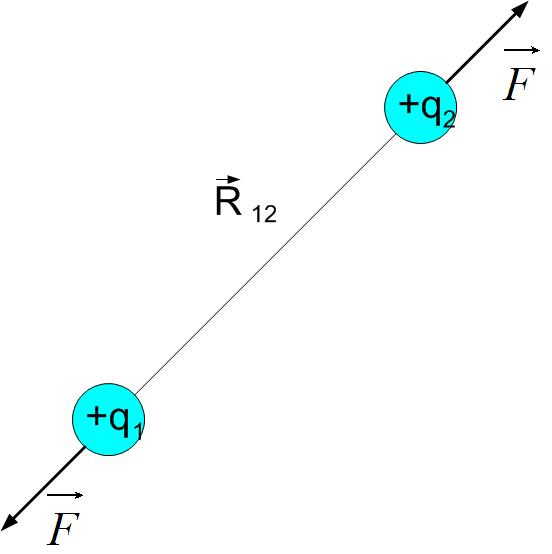
\includegraphics[scale=0.5]{../jpg/Two_Static_Charges.jpg}
\end{center}
\caption{Vector representation of Coulomb's force between two static charges.}
\label{twostaticch}
\end{figure}


\subsection{How perfect is this balance?}

{\bf EXAMPLE} 


Let’s calculate the repulsive force if there was a little bit of unbalance. Say that each of these two tables had 100 extra electrons. Let’s try to calculate the repulsive force. 


Electromagnetic force is one of four we know today. Let’s discover the other forces.


\subsection{Why is it that the atomic nucleus stays together when it is made out of the same kind of matter?}


We just elaborated that if two charges are of the same kind, the electrostatic force will push them away from each other. It seems that there needs to be another kind of force that keeps the nucleus together. This force is called the nuclear force. This is the strongest force, but acts at a short distance. For example if we have a lot of protons in the nucleus such as in radioactive elements the nucleus can split by just lightly tapping it. 

The last force is a weak-interaction force that plays role in radioactive decay. 


\subsection{Which four forces did we talk about today?}

\begin{itemize}
\item Nuclear Force
\item Electromagnetic Force
\item Weak-Interaction Force
\item Gravitational Force.
\end{itemize}

\subsection{Coulomb's Law}

Let’s review the Coulomb's Law that governs the behavior of electrostatic force.

\begin{enumerate}
\item Like charges repel
\item Opposite charges attract
\item The force acts along the line that joins the charges
\item The strength of the force is given by the expression \ref{Coulombslaw}.
\end{enumerate}





\subsection{What’s the difference between the terms force and field?}

Another bunch of questions could be:
\begin{itemize}
\item How do we now if we are in a gravitational field.
\item What is the difference between the gravitational field and gravitational force?
\item More specifically what is the meaning of the term “field” anyway?
\end{itemize}

Let’s try to answer some of these questions.

\subsection{More about the gravitational force and field}

How do we know that we are in the gravitational field and not in zero gravity field? No matter how hard we try to launch ourselves in the outer space by jumping, we still come back to mother earth. If we drop a pencil, where will it go? Why is that so? The gravitational force attracts the pencil (and us).  Another way to say that a gravitational force exists is to say that there is the field of force acting on an object. This is our first answer to the question: What is that term {\bf field} anyways. Let's talk more about fields.

We know that the gravitational force acts at distance. There is no giant muscle that attracts our pencil. Earth induces a gravitational field, it's influence exists at every point in space around it. This phenomenon of direct action on a distance has given rise to the concept of fields.  

Let’s see an example of gravitational force. 

What is the source of the earth's gravitational force? Earth (of course). It would be good if we can define a quantity to show what is the strength of this force at any point in space. 



\begin{figure}[htbp]
\begin{center}
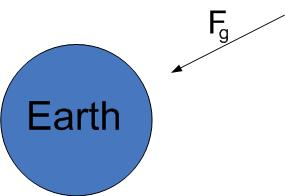
\includegraphics[scale=0.5]{../jpg/earth.jpg}
\end{center}
\caption{Gravitational force.}
\label{wind}
\end{figure}






We can define gravitational field at any point in space through the gravitational force: If an object with mass $m_m$ existed at the point $r$ away from earth, it would experience the force $F_g$, we can say that the gravitational field at that point is equal to

\begin{eqnarray}
\Psi = \frac{\vec{F_g}}{m_m} \\
\Psi = \gamma \frac{m_e}{r^2} \hat{r}
\end{eqnarray} \label{gravitationalfield}


We don’t need the moon in any particular spot to know what would be the gravitational field at that particular point. Note that the field does not depend on the moon’s mass! It depends only on the earth’s mass, gravitational constant and the distance to the point we want to find the field.



\section{Electrostatics}




\subsection{More about the Electrical force and field}

The same situation we have with the electrical force and field. The electric field  is defined as the force that a charge would experience divided by the charge.


\begin{eqnarray}
\vec{E} = \frac{\vec{F_e}}{q_2} \\
\vec{E} =  \frac{q_e}{4 \pi \epsilon_0 r^2} \hat{r}
\end{eqnarray} \label{electricfield}



\begin{figure}[htbp]
\begin{center}
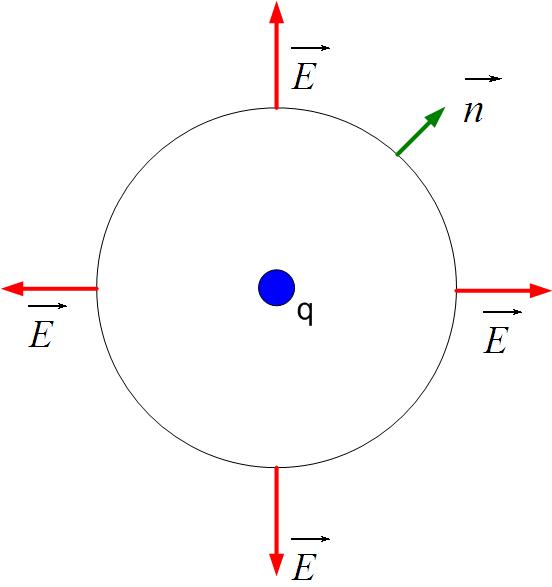
\includegraphics[scale=0.5]{../jpg/unitchargefield.jpg}
\end{center}
\caption{Electric field due to a unit charge q.}
\label{UnitCh}
\end{figure}





What is the source of the electrical force or field? Electric charge (of course). 

\subsection{Properties of Electric Charge}

\subsubsection{Electric charge cannot be created or destroyed.} 

If the total net charge of an object is $q$, and if that object has $n_e$ electrons and $n_p$ protons, then the total charge is $q=n_p e-n_e e$. 

%{\large EXAMPLE}

%An object has 3 protons and 2 electrons. Find what is the net charge of %the object. Assume that the 2 protons and 2 electrons have recombined %(became neutral). What is the net charge now?

\subsubsection{What is the electric field if we have more than one charge?}

The total electric field at a point in space from the two charges is equal to the sum of the electric fields from the individual charges at that point.

%{\large EXAMPLE} Two positive unit charges are fixed in air in Cartesian %coordinate system at points A(0,-1) and B(0,1). Find the electric field %at the points C(0,0) and D(1,1).

\subsubsection{What if the charge is not in air?} 

Let’s look at Coulomb’s law again. 


\begin{eqnarray}
\vec{F_e}=\frac{q_1 q_2}{4 \pi \epsilon_0 r^2} \hat{R_{12}}
\end{eqnarray}\label{Coulombslaw2}
Which quantity in this formula depends on the material? $\epsilon_0$. If the charge is within a dielectric material, then we need to account for that by changing this $\epsilon_0$ somehow. If we place the charge inside a dielectric material what do you think will happen with the atoms in the material? The atoms will get distorted and polarized. Such a polarized atom we call an electric dipole. The distortion process is called polarization. Because the material acts in such a way, the electric field around this point charge is different than if there was no material. In any dielectric medium, the electric field is defined as


\begin{eqnarray}
\vec{F_e}=\frac{q_1 q_2}{4 \pi \epsilon r^2} \hat{R_{12}} \\
\epsilon = \epsilon_0 \epsilon_r
\end{eqnarray}\label{Coulombslaw3}

We added unitless quantity $\epsilon_r$, relative dielectric constant. $\epsilon_r$ values for different materials is shown in one of the tables in the book. Let’s see it’s values for different materials. $\epsilon_r$ varies from 1 (air), to 2.2 (Teflon) to 80 (water). 

Electric field density is the quantity that we introduce here:

\begin{eqnarray}
\vec{D}= \epsilon \vec{E}
\end{eqnarray}


\subsection{Principle of Superposition}

If we have two charges, the total field due to both charges is equal to the vector sum of the fields due to individual charges, see Figure \ref{superposition}.  The field at



\begin{figure}[htbp]
\begin{center}
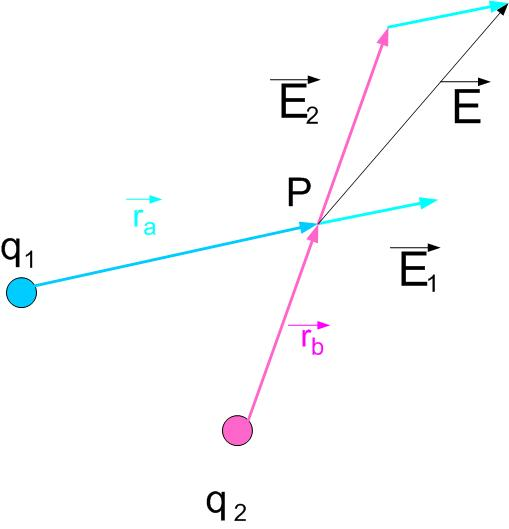
\includegraphics[scale=0.5]{../jpg/superposition.jpg}
\end{center}
\caption{Electric Field due to two charges.}
\label{UnitCh}
\end{figure}

The fields or charges $q_1$ and $q_2$ are:

\begin{eqnarray}
\vec{E_1}=\frac{q_1}{4 \pi \epsilon_{0} {r_a}^2} \hat{r_a} \label{field}\\
\vec{E_2}=\frac{q_1}{4 \pi \epsilon_{0} {r_b}^2} \hat{r_b}
\end{eqnarray}

Where $\hat{r_a}$ and $\hat{r_b}$ are unit vectors in the direction of $r_a$ and $r_b$. The total field due to both charges is


\begin{eqnarray}
\vec{E}=\vec{E_1} + \vec{E_2} 
\end{eqnarray}






\subsection{Electric Field in Rectangular Coordinates}


In general equation for the electric field is given as



\begin{eqnarray}
\vec{E}=\frac{q_1}{4 \pi \epsilon_{0} {r_a}^2} \hat{r_a} \label{genfield}
\end{eqnarray}

The electric field at a point $P(x,y,z)$ due to a charge $q_1$ positioned at a point $P_{q_1}(x_1, y_1, z_1 )$  in the rectangular coordinate system is shown in Figure \ref{singlecharge}. The position vector of the point $P_{q_1}$  is 


\begin{figure}[htbp]
\begin{center}
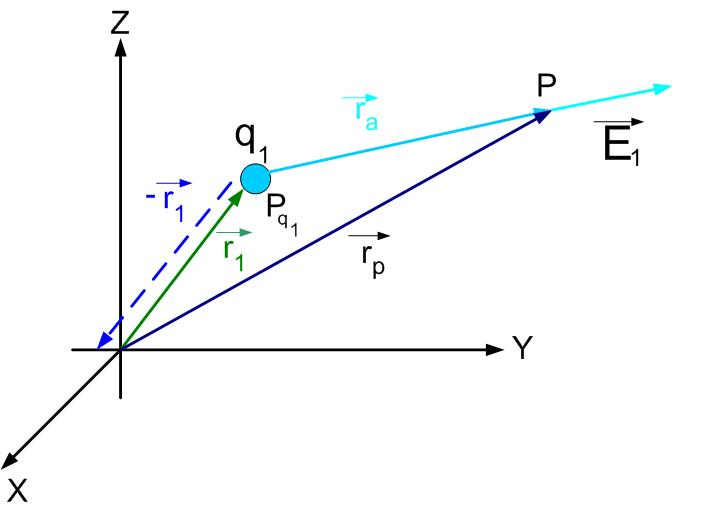
\includegraphics[scale=0.5]{../jpg/singlechargecartcoord.jpg}
\end{center}
\caption{Electric Field due to a unit charge in Rectangular coordinate system.}
\label{singlecharge}
\end{figure}





\begin{eqnarray}
\vec{r_1}=x_1 \vec{x} + y_1 \vec{y} +z_1 \vec{z}
\end{eqnarray}

The position vector of point $P$ is equal to

\begin{eqnarray}
\vec{r_p}=x\vec{x} + y \vec{y} +z \vec{z}
\end{eqnarray}

The two vectors mark the beginning and the end of the distance vector $\vec{r_a}$  between points $P_{q_1}$ and $P$. The vector  $\vec{r_a}$ is the sum of vectors $-\vec{r_p}$ and $\vec{r_1}$



\begin{eqnarray}
\vec{r_a}=\vec{r_p} + (-\vec{r_1})
\end{eqnarray}

When we substitute position vectors $r_1$ and $r_p$:

\begin{eqnarray}
\vec{r_a}= (x - x_1) \vec{x} +(y - y_1) \vec{y} +(z - z_1) \vec{z}
\end{eqnarray}

Vector $\vec{r_a}$ has the magnitude of:


\begin{eqnarray}
|\vec{r_a}|= \sqrt{(x - x_1)^2 +(y - y_1)^2 +(z - z_1)^2}
\end{eqnarray}

Unit vector in the direction of vector $\vec{r_a}$ is:


\begin{eqnarray}
\hat{r_a}= \frac{\vec{r_a}}{|\vec{r_a}|} \\
\hat{r_a}=\frac{\vec{r_a}}{\sqrt{(x - x_1)^2 +(y - y_1)^2 +(z - z_1)^2}}
\end{eqnarray}



\begin{eqnarray}
\vec{E_1}=\frac{q_1}{4 \pi \epsilon_{0} {r_a}^2} \hat{r_a}
\end{eqnarray}

Where $r_a$ is the distance between the charge $q_1$ and the point $P$. Substituting expressions for $\hat{r_a}$, and $|\vec{r_a}|$ in equation \ref{genfield} we get

 



\begin{eqnarray}
\vec{E_1}=\frac{q_1}{4 \pi \epsilon_{0} {\sqrt{(x - x_1)^2 +(y - y_1)^2 +(z - z_1)^2}
}^3} \vec{r_a} \label{eqonecharge}
\end{eqnarray}

Substituting 


For two charges, as shown in Figure \ref{twocharges} equation \ref{eqonecharge} becomes

\begin{eqnarray}
\vec{E}= \frac{q_1}{4 \pi \epsilon_{0} {\sqrt{(x - x_1)^2 +(y - y_1)^2 +(z - z_1)^2}
}^3} \vec{r_a} + \frac{q_2}{4 \pi \epsilon_{0} {\sqrt{(x - x_2)^2 +(y - y_2)^2 +(z - z_2)^2}
}^3} \vec{r_b} 
\end{eqnarray}


\begin{figure}[htbp]
\begin{center}
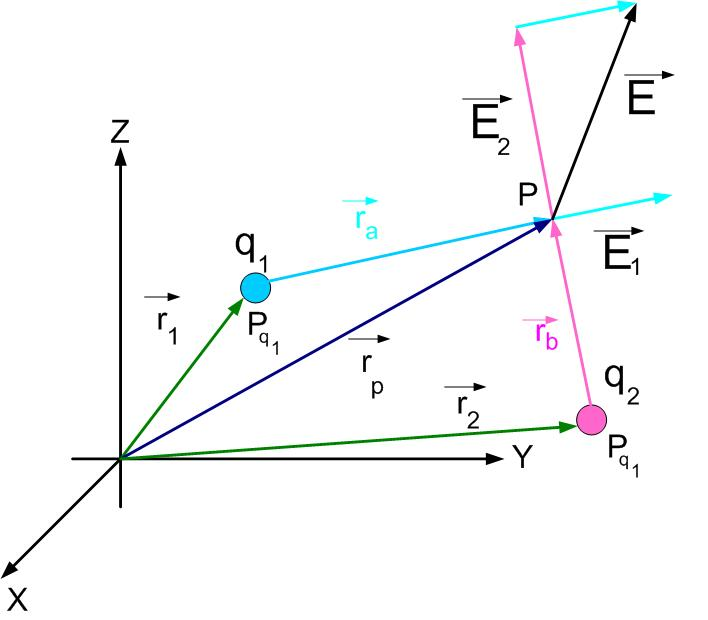
\includegraphics[scale=0.5]{../jpg/twochargescartcoord.jpg}
\end{center}
\caption{Electric field due to two charges in  Rectangular coordinate system.}
\label{singlecharge}
\end{figure}









\subsection{Electric Field Distributions}

{\bf Example of Line Charge Distribution}

Find the field at the z-axis of a loop of charge. Charge is uniformly distributed along the loop with line charge density of $\rho_l$.





\begin{figure}[htbp]
\begin{center}
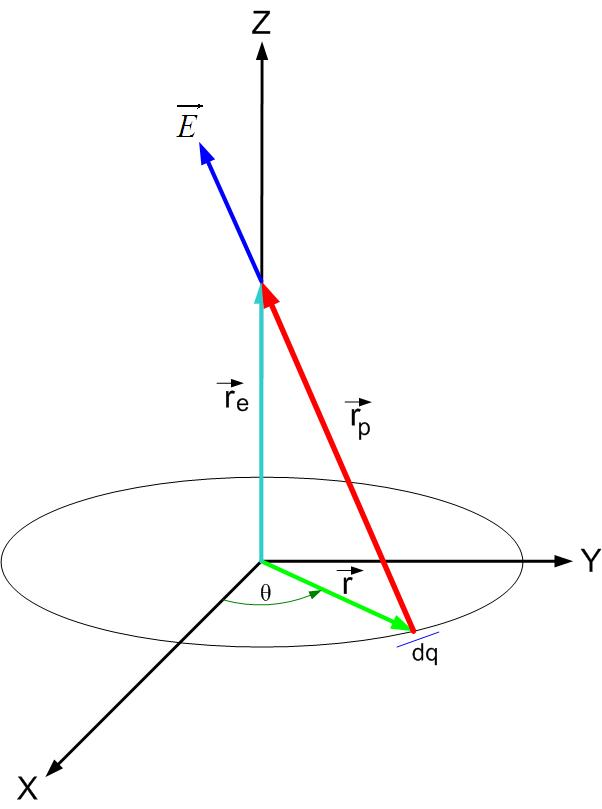
\includegraphics[scale=0.5]{../jpg/chargedistribution.jpg}
\end{center}
\caption{Loop of wire uniformly charged with line charge density $\rho_l$. Electric field is shown due to a very small section of the loop.}
\label{linecharge}
\end{figure}








{\bf Line charge distribution}


{\bf Surface charge distribution}


DISK of charge



\begin{figure}[htbp]
\begin{center}
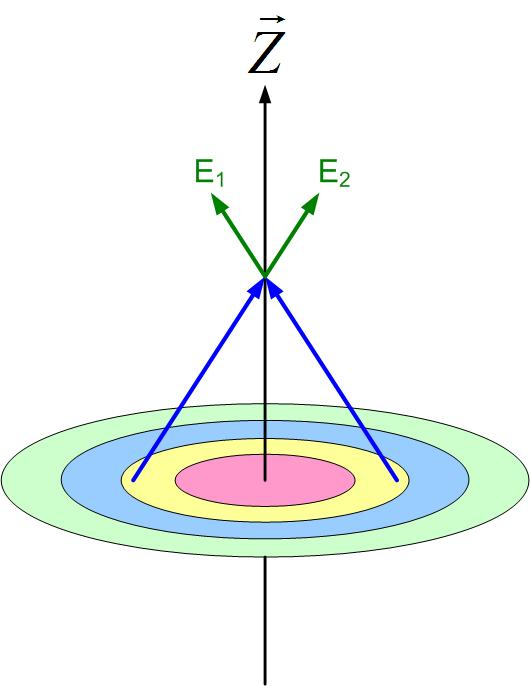
\includegraphics[scale=0.5]{../jpg/surfacedistributiondisk.jpg}
\end{center}
\caption{Disk of charge can be regarded as an infinite number of concentric rings of charge.}
\label{diskcharge}
\end{figure}



Infinite plane


\begin{figure}[htbp]
\begin{center}
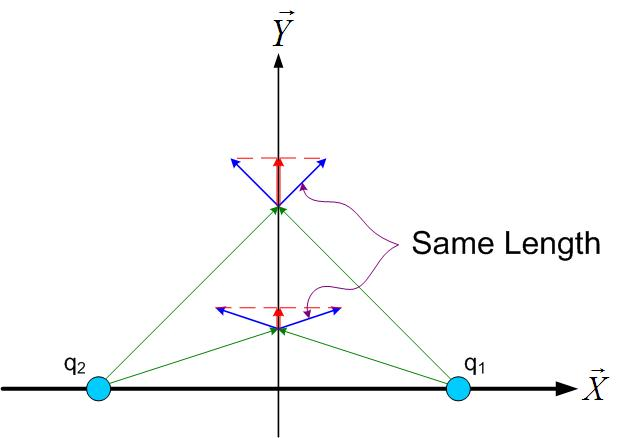
\includegraphics[scale=0.5]{../jpg/constantelectricfieldinfiniteplane.jpg}
\end{center}
\caption{Electric field from two rings located on the infinite plane.}
\label{diskcharge}
\end{figure}





{\bf Volume charge distribution}





{\large EXAMPLE} Line charge distribution Loop of wire

{\large EXAMPLE} Surface charge distribution Disk

{\large EXAMPLE} Volume charge distribution diode


\subsection{Gauss’ Law}




{\large EXAMPLE} Wire


\begin{figure}[htbp]
\begin{center}

\includegraphics[scale=0.5]{../jpg/gausslawwire.jpg}
\end{center}
\caption{Application of Gauss's Law to find Electric Field of wire.}
\label{GausLine}
\end{figure}





{\large EXAMPLE} Infinite Plane


\begin{figure}[htbp]
\begin{center}
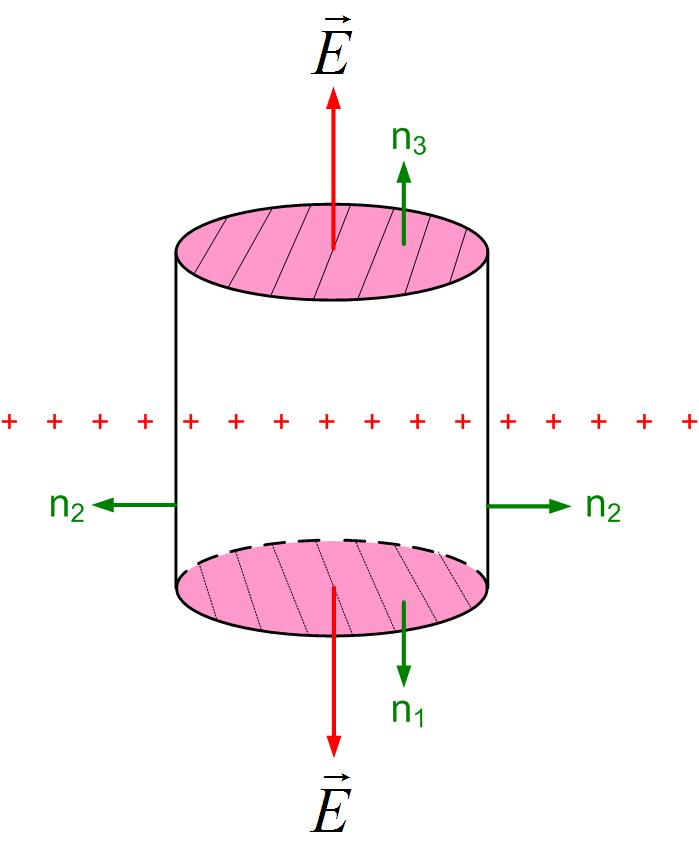
\includegraphics[scale=0.5]{../jpg/infiniteplaneofcharge.jpg}
\end{center}
\caption{Infinite plane charged with positive surface charge density $\rho_S$.}
\label{GausPlane}
\end{figure}




{\large EXAMPLE} Two Infinite Planes




\begin{figure}[htbp]
\begin{center}
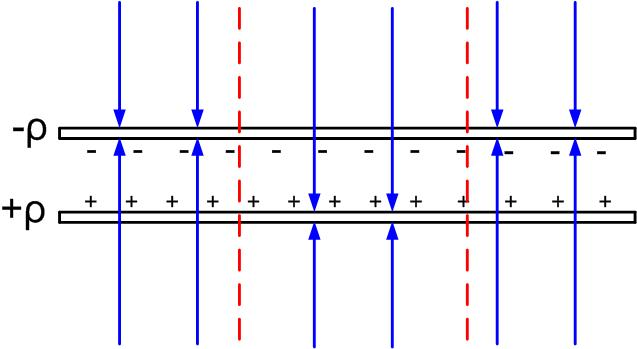
\includegraphics[scale=0.5]{../jpg/infiniteparallelplates.jpg}
\end{center}
\caption{Two infinite planes charged with positive surface charge density $\rho_S$ and $-\rho_S.$}
\label{Gaus2Plane}
\end{figure}





\section{Definition of Potential and Voltage}



\begin{figure}[htbp]
\begin{center}
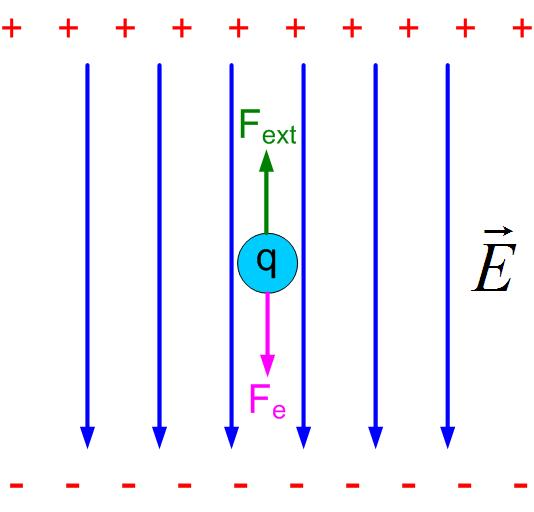
\includegraphics[scale=0.5]{../jpg/potential.jpg}
\end{center}
\caption{Potential}
\label{Potential}
\end{figure}






\begin{figure}[htbp]
\begin{center}
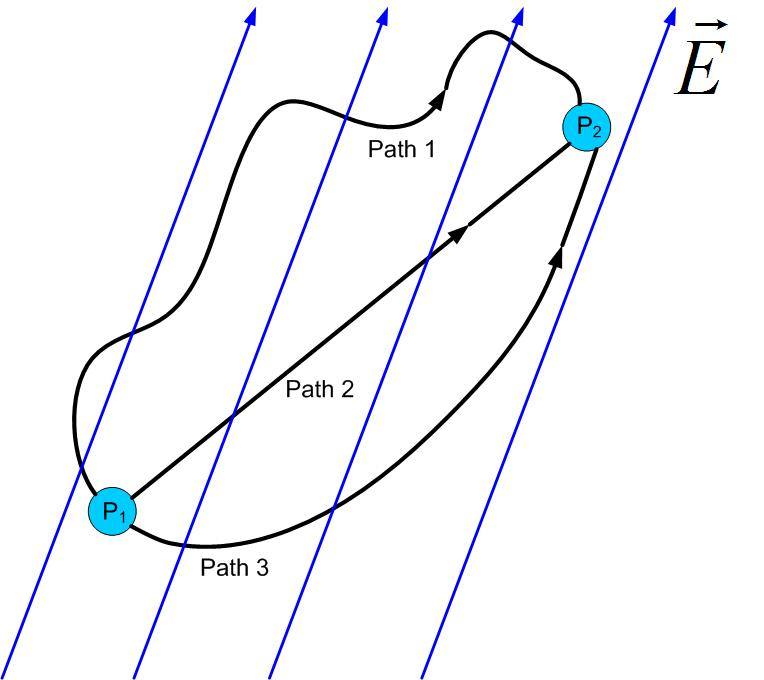
\includegraphics[scale=0.5]{../jpg/workindependentofpath.jpg}
\end{center}
\caption{Potential is not dependent on the specific path.}
\label{PotentialWork}
\end{figure}








{\large EXAMPLE} Potential due to unit charge





\subsection{Capacitance}
What is capacitance, how does it affect circuits.

\subsection{Electric Field inside Metals}


\subsection{Boundary Conditions}




\begin{figure}[htbp]
\begin{center}
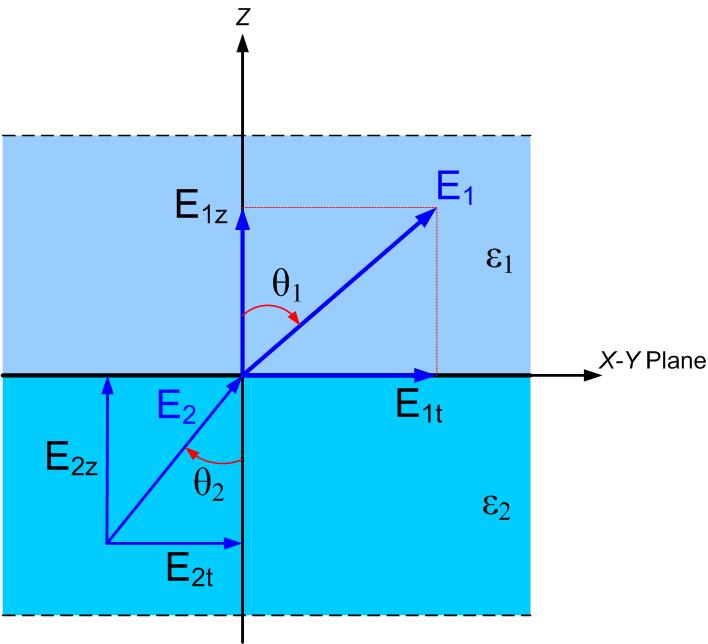
\includegraphics[scale=0.5]{../jpg/boundaryconditions.jpg}
\end{center}
\caption{Boundary Conditions for Electric Field.}
\label{BoundaryCondition}
\end{figure}





\begin{figure}[htbp]
\begin{center}
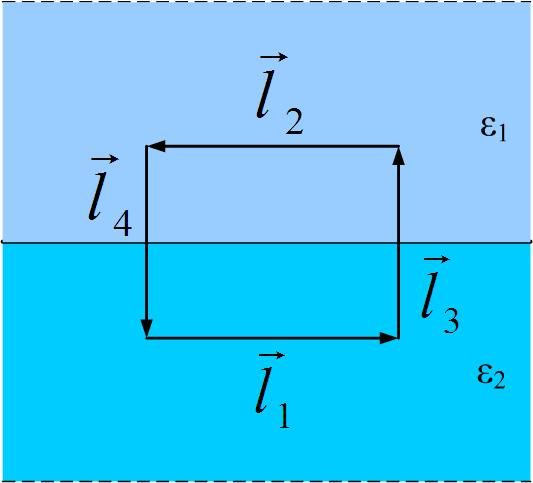
\includegraphics[scale=0.5]{../jpg/integrationpathtangfield.jpg}
\end{center}
\caption{Integration}
\label{BoundaryCondition}
\end{figure}




\begin{figure}[htbp]
\begin{center}
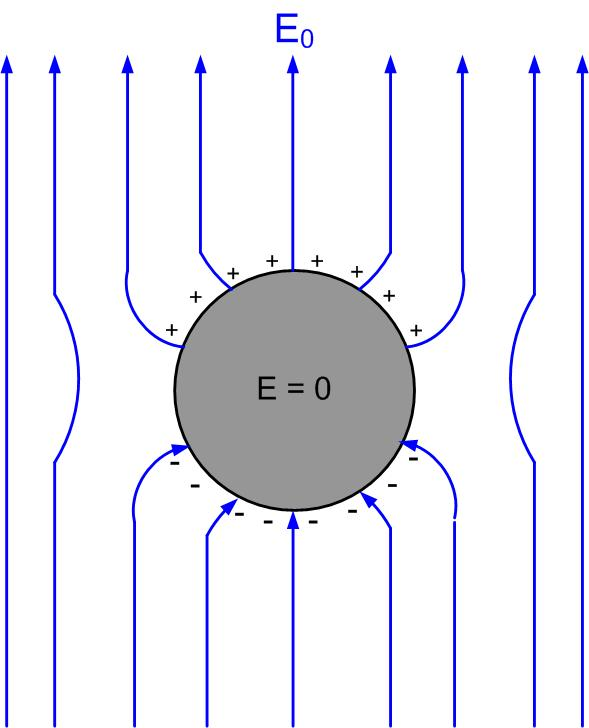
\includegraphics[scale=0.5]{../jpg/metalsphereinefield.jpg}
\end{center}
\caption{Metallic sphere in an external electric field.}
\label{BoundaryConditionMetal}
\end{figure}








\subsection{Image Theory}







\end{document} 
